\documentclass[11pt]{article}
\usepackage[a4paper,margin=2.5cm]{geometry}
\usepackage{amsmath}
\usepackage{enumitem}
\usepackage{hyperref}
\usepackage{amssymb}
\usepackage{graphicx}
\usepackage{amsthm} % for proof environment

\newif\ifshowanswers
% \showanswerstrue % Uncomment to include answers

\title{Exercises on Session 2: Probabilities and Random Variables}
\author{Vasilis Gkolemis}
\date{June 2025}

\begin{document}

\maketitle

\section{Exercise: The expected value of the mean (independent case)}
Let \(X_1, X_2, \ldots, X_n\) be independent random variables. Prove that $Y = \frac{1}{n} \sum_{i=1}^n X_i$ has expected value:

\[
  \mathbb{E}[Y] = \frac{1}{n} \sum_{i=1}^n \mathbb{E}[X_i].
\]
What is the expected value of \(Y\) if all \(X_i\) are coming from the same distribution with expected value \(\mu\)?

\ifshowanswers
  \paragraph{Solution.}

\begin{align*}
  \mathbb{E}[Y] &= \mathbb{E}\left[\frac{1}{n} \sum_{i=1}^n X_i\right] \\
                &= \frac{1}{n} \mathbb{E}\left[\sum_{i=1}^n X_i\right] \\
                &= \frac{1}{n} \sum_{i=1}^n \mathbb{E}[X_i].
\end{align*}

If all \(X_i\) are coming from the same distribution with expected value \(\mu\), then:
\[
  \mathbb{E}[Y] = \frac{1}{n} \sum_{i=1}^n \mu = \mu.
\]

\fi


\section{Exercise: The variance of the mean (independent case)}
Let \(X_1, X_2, \ldots, X_n\) be independent random variables with variances \(\sigma_i^2 = \text{Var}(X_i)\). Prove that the variance of the mean \(Y = \frac{1}{n} \sum_{i=1}^n X_i\) is given by:
\[
  \text{Var}(Y) = \frac{1}{n^2} \sum_{i=1}^n \sigma_i^2.
\]
What is the variance of \(Y\) if all \(X_i\) are coming from the same distribution with variance \(\sigma^2\)?

\ifshowanswers
\paragraph{Solution.}
By the properties of variance and independence, we have:
\begin{align*}
  \text{Var}(Y) &= \text{Var}\left(\frac{1}{n} \sum_{i=1}^n X_i\right) \\
                &= \frac{1}{n^2} \text{Var}\left(\sum_{i=1}^n X_i\right) \\
                &= \frac{1}{n^2} \sum_{i=1}^n \text{Var}(X_i) \\
                &= \frac{1}{n^2} \sum_{i=1}^n \sigma_i^2.
\end{align*}

If all \(X_i\) are coming from the same distribution with variance \(\sigma^2\), then:
\[
  \text{Var}(Y) = \frac{1}{n^2} \sum_{i=1}^n \sigma^2 = \frac{n \sigma^2}{n^2} = \frac{\sigma^2}{n}.
\]

\fi

\section{Exercise: Practical implication of (1) and (2)}

In a test you are asked to find the \textit{expected value} of two probability distributions;
\begin{itemize}
\item the gamma distribution $\Gamma(x; \alpha, \beta)$, where the shape $\alpha = 2$ and the rate $\beta = 3$
\item the beta distribution $B(x; \alpha, \beta)$, where the shape parameters are \(\alpha = 2\) and \(\beta = 5\).
\end{itemize}

\noindent
As you do not remember the closed-form formulas, you rely on a computer with R installed to estimate them.

\begin{enumerate}
\item Write an R script that estimates (a) $\mathbb{E}_X[\Gamma(X; \alpha=2, \beta=3)]$ and (b) $\mathbb{E}_X[B(X; \alpha=2, \beta=5)]$.
\item What is the standard deviation of the approximation? Write an R script that estimates the standard deviation of the approximation.
\item Does the standard deviation makes you confident about the approximation? Are you (almost) sure that the approximation is close enough to the real expected value, within a $\pm 0.1$ interval?
\end{enumerate}

Write an R script that estimates (a) $\mathbb{E}_X[\Gamma(X; \alpha=2, \beta=3)]$ and (b) $\mathbb{E}_X[B(X; \alpha=2, \beta=5)]$.

\paragraph{Hint:}
Use `rgamma(n, shape, rate)` where `n` is the number of samples, `shape` is \(\alpha\), and `rate` is \(\beta\).
Use `rbeta(n, shape1, shape2)` where `n` is the number of samples, `shape1` is \(\alpha\), and `shape2` is \(\beta\).

\ifshowanswers
  \paragraph{Solution.}
  The ground truth solutions are:
  \begin{align*}
    \mathbb{E}_X[\Gamma(X; \alpha=2, \beta=3)] &= \frac{\alpha}{\beta} = \frac{2}{3} \approx 0.6667, \\
    \mathbb{E}_X[B(X; \alpha=2, \beta=5)] &= \frac{\alpha}{\alpha + \beta} = \frac{2}{2 + 5} = \frac{2}{7} \approx 0.2857.
  \end{align*}

\begin{verbatim}
# 1. Estimate expected value of a Gamma(alpha, beta) distribution
alpha <- 2
beta <- 3  # Rate parameter
set.seed(123)
samples_gamma <- rgamma(10000, shape = alpha, rate = beta)
expected_gamma <- mean(samples_gamma)
cat("Estimated expected value of Gamma(", alpha, ",", beta, ") = ", expected_gamma, "\n")

# 2. Estimated variance of the approximation
variance_gamma <- var(samples_gamma)
cat("Estimated variance of the approximation for Gamma distribution = ", variance_gamma, "\n")

# 3. Standard error of the approximation
standard_error_gamma <- sqrt(variance_gamma / length(samples_gamma))
cat("Estimation is: ", expected_gamma, "with +- ", standard_error_gamma, "\n")

# 4. Estimate expected value of a Beta(alpha, beta) distribution
alpha_beta <- 2
beta_beta <- 5
set.seed(123)
samples_beta <- rbeta(10000, shape1 = alpha_beta, shape2 = beta_beta)
expected_beta <- mean(samples_beta)
cat("Estimated expected value of Beta(", alpha_beta, ",", beta_beta, ") = ", expected_beta, "\n")

# 5. Estimated variance of the approximation
variance_beta <- var(samples_beta)
cat("Estimated variance of the approximation for Beta distribution = ", variance_beta, "\n")

# 6. Standard error of the approximation
standard_error_beta <- sqrt(variance_beta / length(samples_beta))
cat("Estimation is: ", expected_beta, "with +- ", standard_error_beta, "\n")
\end{verbatim}

\fi
\section{Exercise: Sample from a more complicated distribution}




Now you are asked to estimate the expected value of the product of a beta and a gamma distribution;
$p(X) = \Gamma(X; \alpha=2, \beta=3) \cdot B(X; \alpha=2, \beta=5)$. Can you write an R script to estimate this expected value? Is it straightforward (like two or three lines of code) or you need to think of something more complicated?

\ifshowanswers
  \paragraph{Solution.}
  It is not straightforward.
  The reason is that the product of two distributions is not a standard distribution (one of these that are implemented in common libraries, like R).
  The product of two distributions is a new unnormalized distribution:
  \[
    p(X) = \frac{\Gamma(X; \alpha=2, \beta=3) \cdot B(X; \alpha=2, \beta=5)}{Z}, \text{ where } Z = \int \Gamma(X; \alpha=2, \beta=3) \cdot B(X; \alpha=2, \beta=5) dX
  \]
  Sampling from this distribution is not straightforward; a common approach is to use importance sampling  as we will see in next sessions.

\begin{verbatim}
h <- function(x) dnorm(x, mean = 3, sd = 1) * dexp(x, rate = 1)

sample_h <- function(n) {
  samples <- c()
  M <- 0.4  # Upper bound on h(x) / g(x) where g is Exp(1)
  while (length(samples) < n) {
    x <- rexp(n, rate = 1)
    u <- runif(n)
    accept <- u < h(x) / (M * dexp(x, 1))  # g(x) = dexp(x, 1)
    samples <- c(samples, x[accept])
  }
  return(samples[1:n])
}

set.seed(42)
samples <- sample_h(1000)
hist(samples, breaks = 40, main = "Samples from Gaussian × Exponential")
\end{verbatim}
\fi

\section{Exercise: Illustration of the Central Limit Theorem in R}

The Central Limit Theorem states that the distribution of the sum (or average) of a large number of independent random variables, regardless of their original distribution, will approximate a Gaussian distribution:

\[
  Y = \frac{1}{n} \sum_{i=1}^n X_i \xrightarrow{d} N(\mu, \sigma^2/n)
\]

Write down an R script that illustrates the Central Limit Theorem by sampling from three different non-Gaussian distributions (a) Uniform, (b) Exponential, and (c) Bernoulli distributions. Then, generate \(n\) many samples of the average of \(n_1\) independent draws from that distribution (e.g., \(n_1=30\)) and plot the histogram of these $n$ averaged samples (average of $n_1$ independent draws).
Plot the histogram of the averaged samples to illustrate the approximate normality predicted by the Central Limit Theorem.

\noindent
Seems quinter intutive, right? In figure \ref{fig:clt_example} you can see the histograms of the original distributions. Will their averaged samples look like a Gaussian distribution? To me at least, it is surpising. Let's see!

\begin{figure}[h]
    \centering
    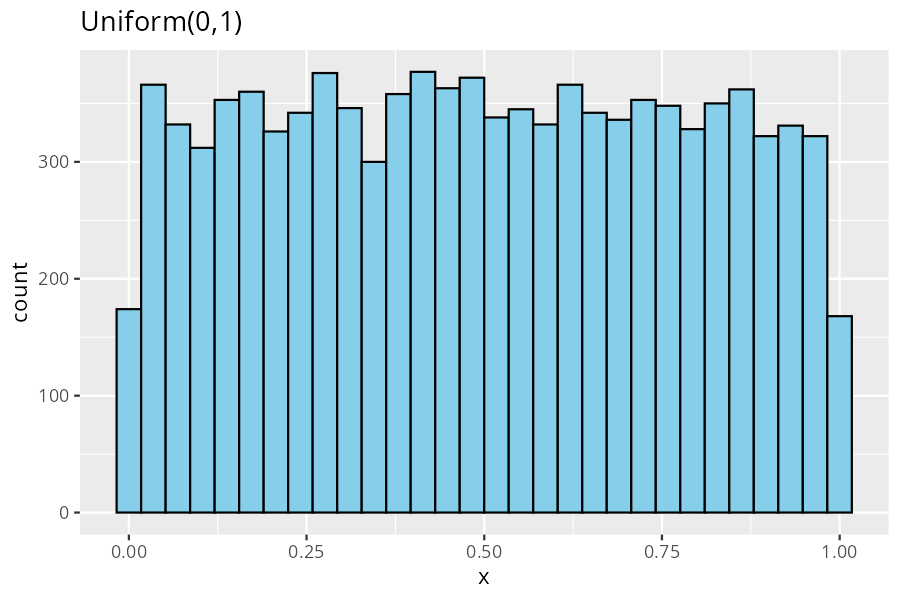
\includegraphics[width=0.32\textwidth]{figures/uniform.png}
    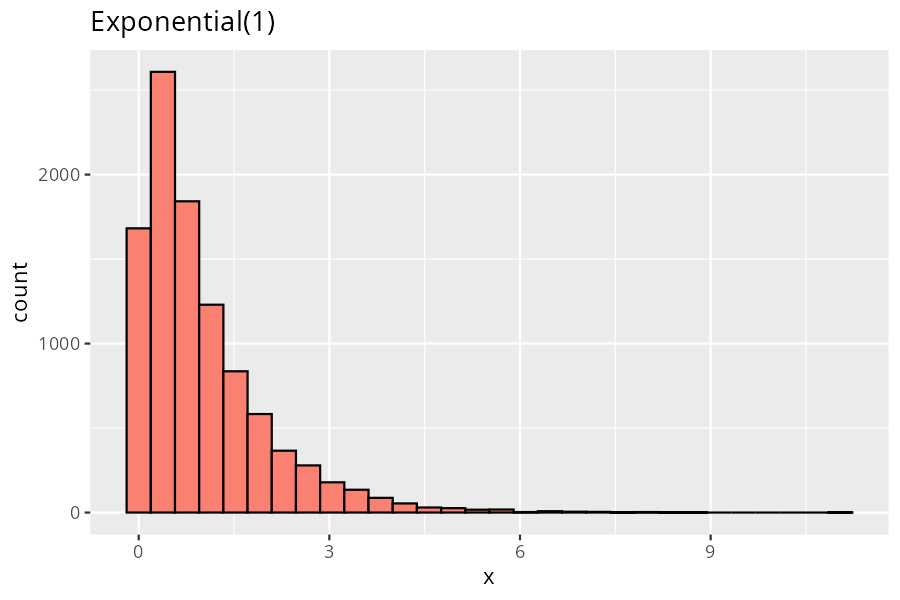
\includegraphics[width=0.32\textwidth]{figures/exponential.png}
    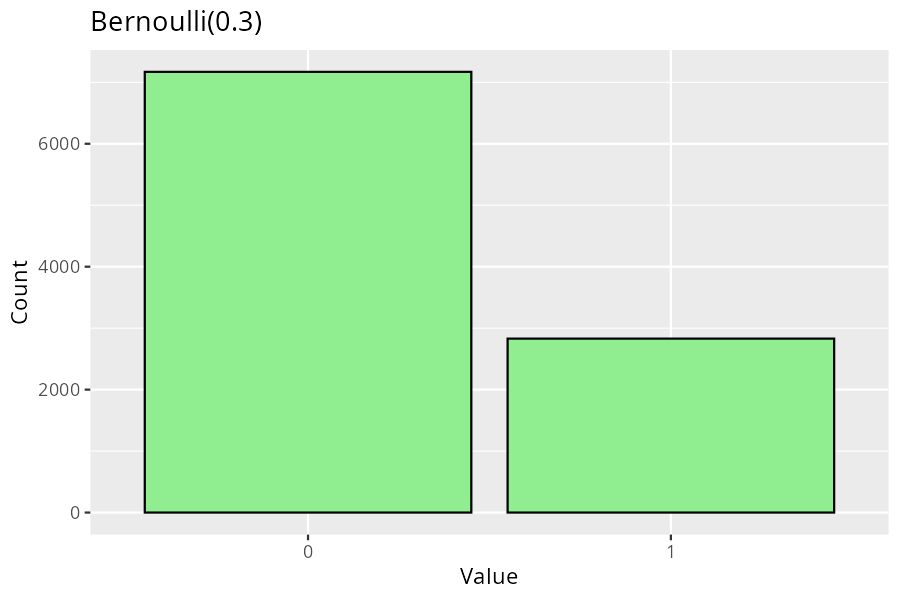
\includegraphics[width=0.32\textwidth]{figures/bernoulli.png}
    \caption{Bernoulli, Uniform, and Exponential distributions (left to right) using $n=10,000$ samples.}
    \label{fig:clt_example}
\end{figure}

\ifshowanswers
  \paragraph{Solution.}

\begin{verbatim}
set.seed(123)

library(ggplot2)
library(gridExtra)

n_samples <- 10000
n_sum <- 30  # number of samples to sum for CLT effect

# 1. Uniform distribution (non-Gaussian)
uniform_samples <- runif(n_samples, min = 0, max = 1)

# 2. Exponential distribution (right-skewed)
exp_samples <- rexp(n_samples, rate = 1)

# 3. Bernoulli distribution (binary, discrete)
bern_samples <- rbinom(n_samples, size = 1, prob = 0.3)

# Plot the original distributions
p1 <- ggplot(data.frame(x = uniform_samples), aes(x)) +
  geom_histogram(bins = 30, fill = "skyblue", color = "black") +
  ggtitle("Uniform(0,1)")

p2 <- ggplot(data.frame(x = exp_samples), aes(x)) +
  geom_histogram(bins = 30, fill = "salmon", color = "black") +
  ggtitle("Exponential(1)")

p3 <- ggplot(data.frame(x = bern_samples), aes(x = factor(x))) +
  geom_bar(fill = "lightgreen", color = "black") +
  ggtitle("Bernoulli(0.3)") + xlab("Value") + ylab("Count")

# Function to compute sums of n_sum samples
clt_samples <- function(x) {
  replicate(n_samples, mean(sample(x, n_sum, replace = TRUE)))
}

# Generate CLT samples
uniform_sum <- clt_samples(uniform_samples)
exp_sum <- clt_samples(exp_samples)
bern_sum <- clt_samples(bern_samples)

# Plot the sums
p4 <- ggplot(data.frame(x = uniform_sum), aes(x)) +
  geom_histogram(bins = 30, fill = "skyblue", color = "black") +
  ggtitle(paste("Sum of", n_sum, "Uniform samples"))

p5 <- ggplot(data.frame(x = exp_sum), aes(x)) +
  geom_histogram(bins = 30, fill = "salmon", color = "black") +
  ggtitle(paste("Sum of", n_sum, "Exponential samples"))

p6 <- ggplot(data.frame(x = bern_sum), aes(x)) +
  geom_histogram(bins = 30, fill = "lightgreen", color = "black") +
  ggtitle(paste("Sum of", n_sum, "Bernoulli samples"))

# Show all plots
grid.arrange(p1, p4, p2, p5, p3, p6, ncol = 2)

# Save images
ggsave(filename = "figures/uniform.png", plot = p1, width = 6, height = 4, dpi = 150)
ggsave(filename = "figures/exponential.png", plot = p2, width = 6, height = 4, dpi = 150)
ggsave(filename = "figures/bernoulli.png", plot = p3, width = 6, height = 4, dpi = 150)
png("figures/clt_demo.png", width = 1200, height = 1600, res = 150)
grid.arrange(p1, p4, p2, p5, p3, p6, ncol = 2)
dev.off()
\end{verbatim}

  \begin{figure}
    \centering
    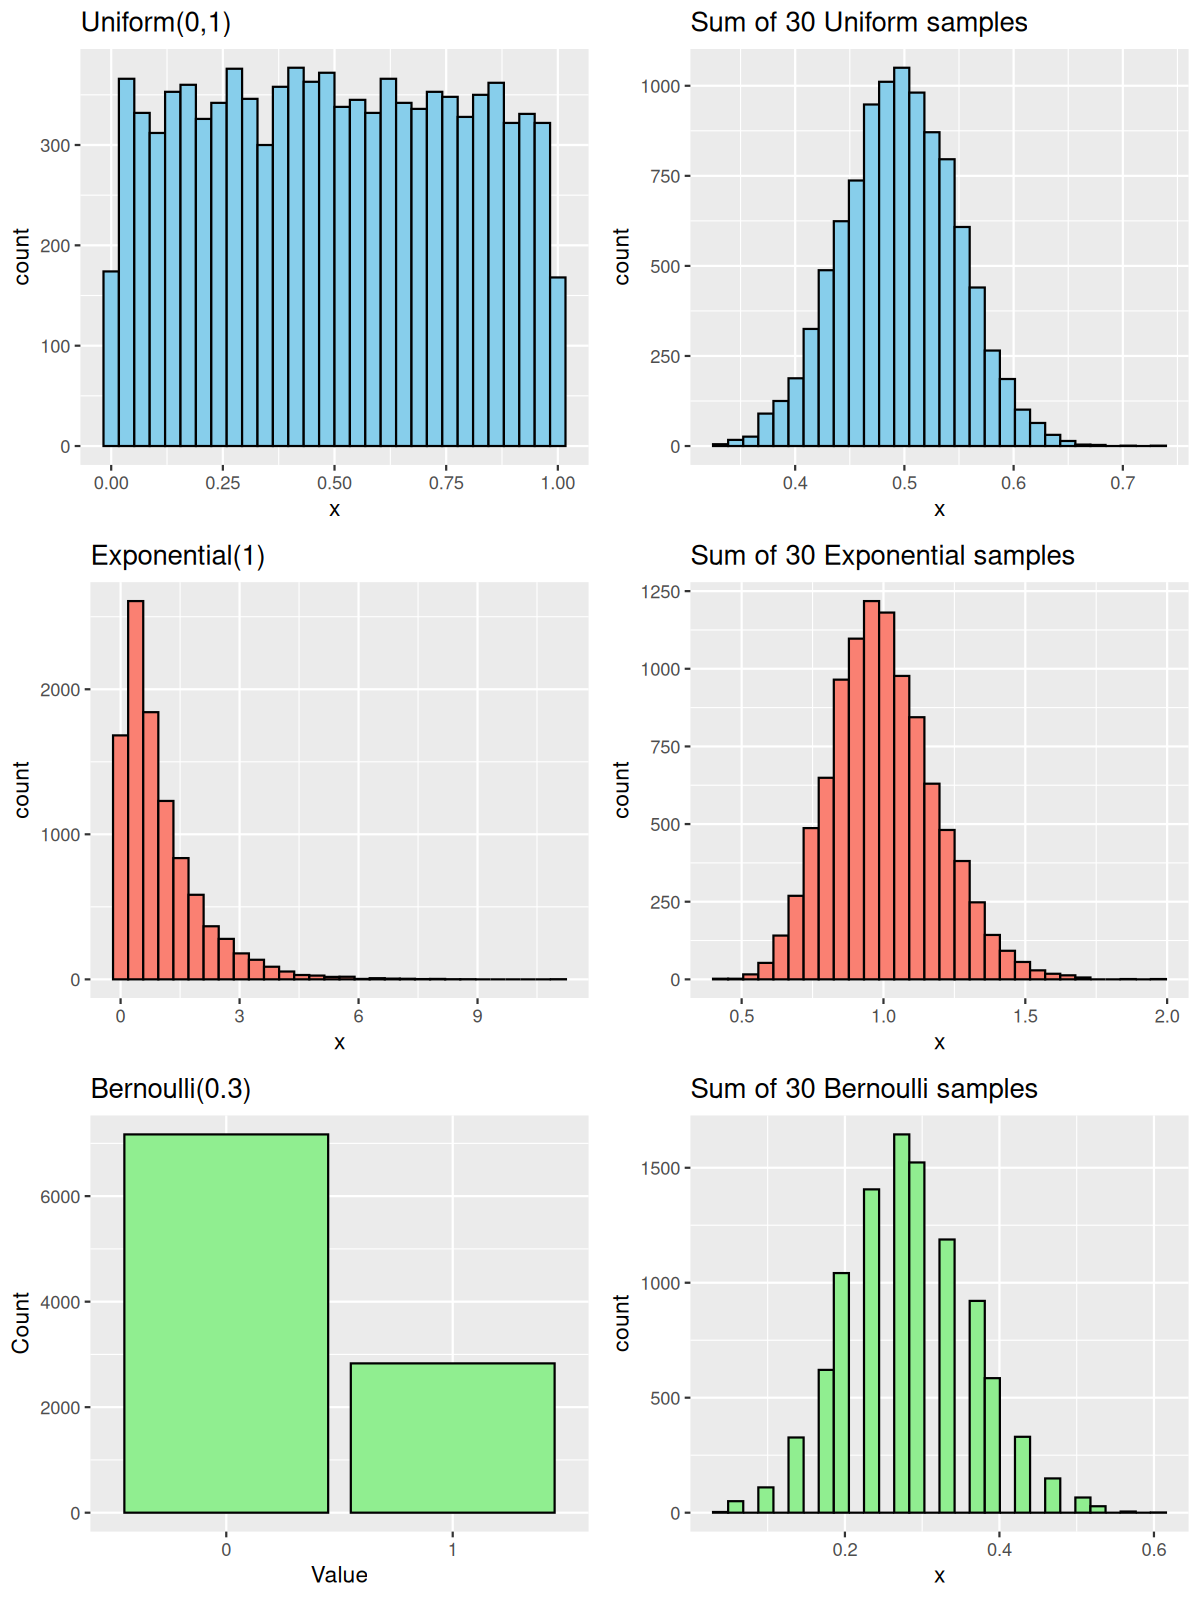
\includegraphics[width=0.8\textwidth]{figures/clt_demo.png}
    \caption{Demonstration of the Central Limit Theorem using Uniform, Exponential, and Bernoulli distributions. The left column shows the original distributions, while the right column shows the distributions of the averages of 30 samples from each distribution.}
    \label{fig:clt_demo}
  \end{figure}

\fi

\end{document}
